\documentclass[tikz]{standalone}

\usepackage{amsfonts}
\usepackage{amsmath}
\usepackage{braket}

\usepackage{tikz}
\usetikzlibrary{calc, decorations, positioning}

% load TikZ grafic definitions
%\input{gfx_TikZ}

% main document
\begin{document}

	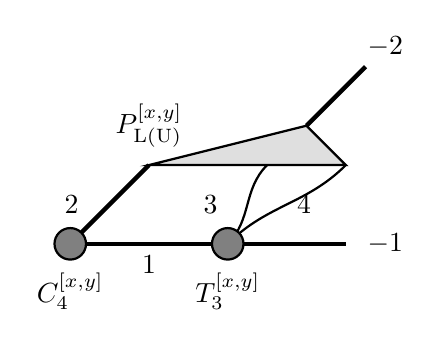
\begin{tikzpicture}[]

		% contant definitions
		\def\ballSize{0.2}

		% tensor network contraction
		\begin{scope}

			% iPEPS network coordinates
			\coordinate (PN) at (+0.0, +0.5);
			\coordinate (PC) at (+0.0, -0.5);

			% CTMRG network coordinates
			\coordinate (C1) at (-0.5, +1.5);
			\coordinate (T1) at (+1.5, +1.5);
			\coordinate (C2) at (+3.5, +1.5);
			\coordinate (T2) at (+2.0, +0.0);
			\coordinate (C3) at (+0.5, -1.5);
			\coordinate (T3) at (-1.5, -1.5);
			\coordinate (C4) at (-3.5, -1.5);
			\coordinate (T4) at (-2.0, -0.0);
			
			% projector P_{LU}
			\begin{scope}[shift = {(-1.00, +0.00)}]
				\coordinate (PUL) at (-1.50, -0.50);
				\coordinate (PUM) at (+0.00, -0.50);
				\coordinate (PUR) at (+1.00, -0.50);
				\coordinate (PUU) at (+0.50, +0.00);
				\node[] at (-1.50, -0.00) {$P_\text{L(U)}^{[x, y]}$};
			\end{scope}

			% tensor labels
			\node[below = 0.25] at (C4) {$C_{4}^{[x,y]}$};
			\node[below = 0.25] at (T3) {$T_{3}^{[x,y]}$};

			% external links
			\draw[ultra thick] (PUU) to ($(PUU) + (+0.75, +0.75)$) node at ($(PUU) + (+1.00, +1.00)$) {$-2$};
			\draw[ultra thick] (T3) to ($(T3) + (+1.50, +0.00)$) node at ($(T3) + (+2.00, +0.00)$) {$-1$};

			% projector
			\draw[thick, fill = gray!25] (PUL) to (PUR) to (PUU) -- cycle;

			% internal links
			\draw[ultra thick] (C4) -- (PUL) node[left = 0.25] at ($(C4)!0.5!(PUL)$) {$2$};
			\draw[ultra thick] (C4) -- (T3) node [midway, below] {$1$};
			\draw[thick] (T3) to [out = 45, in = 225] (PUM) node[left = 0.25] at ($(T3)!0.5!(PUM)$) {$3$};
			\draw[thick] (T3) to [out = 45, in = 225] (PUR) node[right] at ($(T3)!0.5!(PUR)$) {$4$};

			% CTMRG tensors
			\foreach \tensor in {T3, C4} {
				\draw[thick,black,fill = gray] (\tensor) circle (\ballSize);
			}
			
		\end{scope}

	\end{tikzpicture}

\end{document}
%%% Local Variables:
%%% mode: latex
%%% TeX-master: t
%%% End:
